\documentclass[CJK, 12pt, hyperref, bookmark]{z-article}
\usepackage[vmargin=3cm]{geometry}
\usepackage{z-filetree}
\usepackage{float}
\usepackage{verbatim}
\usepackage{environ}
\usepackage{fancyvrb}
\usepackage{mdframed}
\usepackage{fontawesome}
\usepackage{z-tabbrow2}
\pretocmd{\subsection}{\clearpage}{}{}

\usepackage{fancyhdr}
    \pagestyle{fancy}
    \fancypagestyle{plain}

    \fancyhead[LO,RE]{\slshape \sdef (版本 1.4.2)}
    %\fancyhead[LE,RO]{\slshape \leftmark}
    \fancyfoot[C]{}
    \fancyfoot[LO,RE]{}
    %\fancyfoot[LE,RO]{\thepage}

    % 要求页码必须在右上角
        \fancyhead[LE,RO]{\slshape \thepage}
        \fancyfoot[LE,RO]{}

\newcommand\code[1]{\texttt{#1}}

\usepackage{stmaryrd}
\usetikzlibrary{shapes, shadows}
\tikzset{
    win button/.style = {
        fill, rectangle, color=white,fill=gray,
		text width=0.7em, text height=0.6em, 
		align=center, anchor=north east, xshift=-1pt },
}

\newcommand\console[2]{
    \begin{center}
    \begin{tikzpicture}[framed]
	    \node[draw, color=white, rectangle split, rectangle split parts=2, 
	            text width=35em] (comp) at (0,0) {
		    \large \textbf{#1}
		    \nodepart[color=black]{two}
		    \texttt{#2}
	    };
	    \begin{scope}[start chain=going above left, node distance=0pt]
		    \draw (comp.north east) ++(-1pt, -1pt) coordinate(close-corner);
		    \node[on chain, win button] (close) at (close-corner) { \faRemoveSign };
		    \node[on chain, win button] (max) { \faChevronUp };
		    \node[on chain, win button] (min) { \faChevronDown};
	    \end{scope}

	    \draw (comp.north west) rectangle (comp.south east);
	    \begin{scope}[on background layer]
		    \fill[black] (comp.north west) rectangle (close.south east);
	    \end{scope}
    \end{tikzpicture}
    \end{center}
}

\DefineVerbatimEnvironment{codeblk}{Verbatim}{
  frame=single,
  framerule=0.5mm,
  rulecolor=\color{green!20!black},
  numbers=left
}

\newcommand\syntax[1]{
  \begin{mdframed}[
      linecolor=brown,
      linewidth=2pt,
    ]
    #1
  \end{mdframed}
}

\newcommand\sdef{神盾Linux服务器安全卫士}
\newcommand\sdcom{海宁神盾网络信息技术有限公司}
\newcommand\configdir{\texttt{/etc/execfilter.d/}}

\setlength{\parskip}{\baselineskip}

\title {使用说明书 \\ 神盾Linux服务器安全卫士 (版本 1.4.2)}
\author{谢继雷 \\ \sdcom}

\AtBeginDocument{\setuptabsatright}

\begin{document}

    \maketitle
    \clearpage

\section {简介}

    随着 Linux 在服务器市场日益广泛的推广和普及,Linux 服务器正面临着日益严峻的安全风险。许多 Linux 应用存在着不可知的后门程序,这些程序难以检测,危害极大,需要一种更积极的防范策略来控制这些程序对系统关键资源的访问。

    \sdef 采用启发式进程监控技术能够有效避免一大类基于后门的入侵行为。在传统的 Linux 进程安全实践中主要是可执行位 (execution bit) 、SELinux 进程策略等,它们需要服务器管理员对 Linux 的深刻理解和精确的配置才能有效使用,这在安全管控方面可能是很大的开销,并且具有很大的不确定性。

    \begin{figure}[h]
        \centering
        \begin{tikzpicture}[framed]
            \tikzset{
	            fb item/.style = {
		            draw, rectangle, rounded corners=2pt, 
		            fill=white, drop shadow, align=center, },
	            fb hacker/.style = {
		            fb item, },
                fb-c/.style = {
		            fb item, },
	            fb-s/.style = {
		            fb item },
	            fb sdef/.style = {
		            fb-s },
            }
	        \begin{scope}[
		            start chain=going below, node distance=1.5em,
		            every node/.style={on chain, join},
		            every join/.style={->}, ]
	            \node[fb hacker]
		            (hacker) {黑客};
	            \node[fb-c, below of=hacker]
		            (browser) {Web浏览器};
	            \node[fb-s, below of=browser]
		            (fw) {HTTP防火墙};
	            \node[fb-s, below of=fw]
		            (server) {服务器进程};
	            \node[fb item, below of=server]
		            (pm) {进程管理程序};
	            \node[fb item, below of=pm]
		            (target) {目标进程};
	            \node[fb item, below of=target]
		            (system) {系统关键资源};
	        \end{scope}

	        \node[fb sdef, right of=pm, anchor=west, xshift=8em, text width=8em]
		        (sdef) {\sdef};
	        \node[fb item, above right of=sdef, anchor=south west, yshift=2em]
		        (rules) {进程访问规则库};
	        \node[fb sdef, below right of=sdef, anchor=north west, text width=8em]
		        (updater) {\sdef 安全检测中心};
            
            \path[<->] (sdef) edge node[above] {监控} (pm);

	        \draw[->] (rules) .. controls ++(-6em, 0) .. (sdef);
	        \draw[->] (updater) .. controls ++(3em, 6em) .. (rules);
        \end{tikzpicture}
        \caption{\sdef 功能结构图}
    \end{figure}

    在大型机房中,集中式配置是必需的。通过采用中央管理和部署,机房和安全检测防范中心可以建成快速的信息通道,在第一时间阻止入侵者、病毒、软件漏洞的扩散,降低机房的安全威胁,从而有效地提高服务器的可用性。

    \sdef 支持集中化的安全管理。这是通过和 \sdcom安全防控中心合作完成的。当新的漏洞、木马被确认后,\sdcom安全防控中心将形成有效的监控规则并分发给已注册的用户服务器。用户服务器收到通知后会立即重新配置服务,以避免被新型的漏洞、木马等程序入侵。
    
\section {安装}

    插入 \sdef 安装光盘,在文件管理器中找到光盘对应的目录:
    
    \begin{center}
        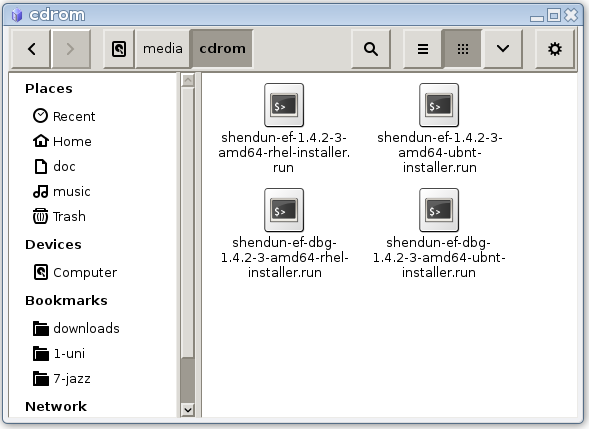
\includegraphics[scale=0.5]{filebrow.png}
    \end{center}
    
    其中不同机型对应有不同的安装程序:
    
    对于 RedHat, RHEL, CentOS 等使用 RPM 包管理程序的 Linux 发行版,
    请选择带有 -rhel- 的安装程序。
    
    对于 Debian, Ubuntu, Mint 等使用 Apt 包管理程序的 Linux 发行版,
    请选择带有 -ubnt- 的安装程序。
    
    对于32位操作系统,请选择带有 -i386- 的安装程序。
    
    对于64位操作系统,请选择带有 -amd64- 的安装程序。
    
    您必须使用 root 用户安装本软件。如果系统采用了 sudo 提权机制,请确保您在 sudoers 中,并在要运行的命令前添加 sudo 前缀。
    
    如果您没有桌面操作系统,请在终端命令行中运行正确的安装程序。
    
    \console{Root Console}{
        \# cd /media/cdrom \\
        \# ls -l \\
        total 2704 \\
        -rwxr-xr-x 1 root 655266 Apr 30 15:51 shendun-ef-1.4.2-3-amd64-rhel-installer.run \\
        -rwxr-xr-x 1 root 609449 Apr 30 15:51 shendun-ef-1.4.2-3-amd64-ubnt-installer.run \\
        -rwxr-xr-x 1 root 786832 Apr 30 15:51 shendun-ef-dbg-1.4.2-3-amd64-rhel-installer.run \\
        -rwxr-xr-x 1 root 711898 Apr 30 15:51 shendun-ef-dbg-1.4.2-3-amd64-ubnt-installer.run \\
        \# ./shendun-ef-1.4.2-3-amd64-ubnt-installer.run \\
        Verifying archive integrity... All good. \\
        Uncompressing shendun-ef installer (deb)  100\% \\
        ... \\
        \phantom
    }
    
    如果所选择的安装程序与当前正在使用的 Linux 操作系统不兼容,安装程序将报错并退出,
    并不会损坏操作系统。
    
    在 SSH 会话中安装本软件具有一定的风险性,如果安装失败或者 \sdef 与安装的机器偶然出现
    不兼容的情况,您可能会出现 SSH 服务关闭并无法登录的困难。如果服务器所在的机房在距离
    非常远的异地,这可能会引起极大的不便。
    
    如果您必须要通过 SSH 的方式安装本软件,建议您在安装本软件的之前多开几个 Root 权限
    的 SSH 会话,并在安装发生异常的时候用另一个 SSH 会话紧急删除本软件:
    
    \console{SSH Console 1}{
        \$ cd /media/cdrom \\
        \$ sudo ./shendun-ef-1.4.2-3-amd64-ubnt-installer.run \\
        ... \\
        \$ sudo -i \\
        Segmentation fault \\
        (session closed) \\
        \vskip 2em \phantom
    }
    
    上面这个例子中,用于安装本软件的 SSH 因为故障而无法提权至 root,这个时候用第二个
    SSH 来恢复系统:
    
    \console{SSH Console 2}{
        \# cd /etc \\
        \# rm ld.so.preload \\
        \# \\
        \vskip 2em \phantom
    }
    
    系统恢复后,在找到问题以前,您可在类似的机型或虚拟机中进行安装调试工作,以免
    影响系统的可用性。
    
    如果您的系统上正运行着需要监控的相关服务,您需要重新启动这些服务,以便将它们置于
    \sdef 的监控下。您可以重新启动服务器以简化这一过程。
    
    如果服务器重新启动后出现严重错误,或者无法启动,请参考后面的故障与解决。
    
\section {卸载}
    
    在 Debian, Ubuntu, Mint 等使用 Apt 包管理程序的 Linux 系统中,运行如下命令以卸载本软件:

    \console{Root Console}{
        \# apt-get purge shendun-ef \\
        Reading package lists... Done \\
        Building dependency tree \\
        Reading state information... Done \\
        The following packages will be REMOVED: \\
        \hskip 1em  shendun-ef* \\
        0 upgraded, 0 newly installed, 1 to remove and 169 not upgraded. \\
        After this operation, 413 kB disk space will be freed. \\
        Do you want to continue? [Y/n] \\
        (Reading database ... 413688 files and directories currently installed.) \\
        Removing shendun-ef (1.4.2-3) ... \\
        Purging configuration files for shendun-ef (1.4.2-3) ... \\
        Processing triggers for man-db (2.6.7.1-1) ... \\
        Processing triggers for libc-bin (2.18-4) ... \\
        \# \\
    }
    
    在 RedHat, RHEL, CentOS 等使用 RPM 包管理程序的 Linux 系统中,运行如下命令以卸载本软件:
    
    \console{Root Console}{
        \# yum remove shendun-ef \\
        Loaded plugins: fastestmirror \\
        Setting up Remove Process \\
        Resolving Dependencies \\
        --> Running transaction check \\
        ---> Package shendun-ef.i386 0:1.4.3-4 set to be erased \\
        --> Finished Dependency Resolution \\
        Dependencies Resolved \\
        =========================================== \\
         Package    Arch  Version  Repository Size \\
        =========================================== \\
        Removing: \\
         shendun-ef i386  1.4.3-4  installed  326 k \\
        Transaction Summary \\
        =========================================== \\
        Remove    1 Package(s) \\
        Reinstall   0 Package(s) \\
        Downgrade   0 Package(s) \\
        Is this ok [y/N]: y \\
        Downloading Packages: \\
        Running rpm_check_debug \\
        Running Transaction Test \\
        Finished Transaction Test \\
        Transaction Test Succeeded \\
        Running Transaction \\
          Erasing        : shendun-ef            1/1 \\
        Removed: \\
          shendun-ef.i386  0:1.4.3-4 \\
        Complete! \\
        \#
    }

\section {配置}

    \sdef 使用配置文件来描述作用于具体应用程序的监控规则。这些配置文件在 \configdir 目录下。
    各个规则项之间不存在依赖关系,配置文件的装载顺序是任意的。

    空行和以 ``\#'' 开头的注释将会被忽略。每条语句以换行符结尾。

    一个配置文件中可以含有多个段,每个段描述了作用于调用者进程的执行规则。监控规则是可以被子进程继承的,
    如果规则描述一个目标程序被父进程拦截了,那么那个目标程序也将会被该父进程的所有子孙进程所拦截。
    
    通常情况下,修改配置文件将立即起作用。但服务进程因为存在缓存,在重新启动前进程控制规则将不会更新。
    尽管如此,一些服务器如 Apache Http 服务器总是通过 Shell 来创建新的进程,因此可以在不重启服务的
    情况下就能立即更新配置。
    
    让我们从一个简单的例子开始配置文件的书写吧!
    
    \subsection {一个简单的例子}
        
        在这个例子中,游戏 foo-game 可能含有后门程序,这条规则用于防止其创建 shell:

        \console{Root Console}{
            \# cat /etc/execfilter.d/games \\
            for /usr/bin/foo-game \\
                deny /bin/sh \\
            \# \\
            \vskip 2em \phantom
        }

        简单吧! 
        
        \sdef 会读取 \configdir 目录下的所有配置文件(但不含子目录),检查文件的格式,
        并合并作用于相同调用者进程的规则。如果当前进程要创建一个进程,而在配置文件中这个被创建的进程是
        被阻止的,那么进程创建就会失败。

        掌握了这个简单的例子后,您现在可以系统的学习一下 \sdef 的综合语法了。
        
    \subsection {for 语句}

    \syntax{
      ``for'' \textit{<应用程序路径>}
    }

    \code{for} 语句指定后续的规则将会作用在哪个应用程序上。\textit{应用程序路径} 必须是绝对路径,
    不带任何引号 ('、")。 路径前后的空格会被忽略,因此,您不能指定文件名头、尾含有空格的应用程序。

    \begin{codeblk}
      for APP1
      ...
      ... (规则只对 APP1 有效)
      ...
      for APP2
      ...
      ... (规则只对 APP2 有效)
      ...
      for APP1
      ...
      ... (规则只对 APP1 有效,并和前面的 APP1 的规则合并。)
      ...
    \end{codeblk}

    同一个应用程序可以分别在不同配置文件、或同一个配置文件中的不同段中多次出现。解析器将会把它们合并。
    当规则数目庞大时,您可以用一种自然的分类的方式来管理这些规则。

    在 \sdef 用这些 \code{for} 规则去匹配调用者进程时,首先会将调用者进程的路径正规化。也就是说
    符号连接会被展开,相对路径会转换成绝对路径。因此这里的应用程序路径必须是绝对路径,并且不要使用符
    号连接。否则这些规则会因为无法匹配而不能产生正确的效果。
    
    虽然相对路径有时也能产生正确的结果,但基于安全考虑,请尽量实用绝对路径。
    
    \subsection {default 语句}

    \code{default} 语句用于说明当没有规则可以匹配目标进程时,调用者进程所表现的默认行为:

    \syntax {
      ``default'' \{ ``allow'' | ``deny'' \}
    }

    仅有两种形式: \code{default allow} 和 \code{default deny}。

    如果您忽略了 \code{default} 语句,默认位 \code{default allow}。

    与其它规则不同的是,\code{default} 是不可继承的。也就是说,如果调用者进程和它的祖先进程中,
    当有多条规则可以匹配目标进程时,各个祖先进程的 \code{default} 行为可以是不同的。当任何一个
    祖先进程在它的 \code{default} 行为以及那个祖先进程做为调用者进程所对应的规则集阻止了目标进
    程,那么目标进程就无法被创建。

    \code{default allow} 规则又称为“白名单”模式,除了规则所列出的项目被允许通过外,其它未定义的项目
    都会被拒绝。这种模式相对于“黑名单”模式的 \code{default deny} 会更安全。但是您需要在简单性和安全
    性之间做出权衡。过度强调安全性也可能会降低服务的可用性,没有可用的服务也就谈不上安全了。
    
    \subsection {allow/deny 语句}

    \syntax {
      \{ ``allow''| ``deny'' \} \textit{<目标进程>}
    }

    \code{allow} 和 \code{deny} 语句用于定义 \sdef 如何处理目标进程的执行请求。

    \console{Root Console}{
        \# cat /etc/execfilter.d/myrules \\
        for /usr/bin/warcraft \\
        \hskip 2em default deny \\
        \hskip 2em allow /sbin/ifconfig \\
        \phantom \\
        for /usr/bin/btdownloader \\
        \hskip 2em deny /sbin/pm-suspend \\
        \hskip 2em deny /sbin/shutdown \\
        \# \\
        \vskip 2em \phantom
    }

    以上的例子显示了,对于游戏应用程序 \code{/usr/bin/warcraft},它可以创建
    \code{/sbin/ifconfig} 进程, 因为这个游戏可能需要 \code{ifconfig} 来启动网络游戏联机, 
    而其它的一切都将被阻止。然而,\code{/usr/bin/btdownloader} 则采用了相反的 \code{default}
    模式,除了 \code{/sbin/pm-suspend} and \code{/sbin/shutdown} 被允许外,其它都将被阻止。
    这是为了防止下载器在下载完成后意外的关机。

    \textit{目标进程} 指定了要执行的目标程序。不同于 \code{for}-语句,它可以是符号链接和相对路径,
    在读入配置文件后,它们将被 \sdef 正规化。如果 \textit{目标进程} 在 PATH 环境变量所列举的目录中,
    可以忽略它们的目录名称。但基于安全考虑,建议您尽可能实用绝对路径。

\section {日志分析}

    \sdef 将进程的访问记录在日志文件中,日志文件位于 /var/log/execfilter.log。每个一段时间,
    系统会将过往已久的日志打包存档,以减少对系统磁盘的空间占用。
    
    在不同操作系统中,\sdef 的日志可能会有差别。在新版本的 Debian 或 Ubuntu 上,系统使用 
    rsyslog-7.x.x 记录日志,在另一些早期版本中,系统可能使用 rsyslog-5.x.x 或 ksyslog 来记
    录日志。这些日志系统的格式和功能不尽相同。在可能的情况下,您应该使用新版的日志系统以便能得到更直观
    和翔实的日志内容。
    
    要访问进程监控日志,您需要 root 身份。
    
    在 rsyslog-7.x.x 日志系统中,您可能会看到如下所示的内容:
    
    \console{Root Console}{
        \# cd /var/log \\
        \# tail execfilter.log \\
        Apr 23 07:18:12 [execfilter] NOTICE:  进程允许:/usr/sbin/exim4 -> /usr/sbin/exim4 \\
        Apr 23 07:44:19 [execfilter] NOTICE:  进程允许:/sbin/start-stop-daemon -> /bin/sh \\
        Apr 23 07:44:19 [execfilter] NOTICE:  进程允许:/bin/dash -> /usr/bin/xargs \\
        Apr 23 08:11:10 [execfilter] NOTICE:  进程被拦截: /usr/sbin/apache2 -> /sbin/reboot \\
        Apr 23 08:12:41 [execfilter] NOTICE:  进程被拦截: /usr/sbin/apache2 -> /sbin/shutdown \\
        \# \\
        \vskip 2em \phantom
    }

    这里,日志的字段依次为:进程创建的时间(月,日,时、分、秒),监控程序,消息的等级(这里是NOTICE,表示重要通知),进程拦截与否和相关进程的具体名称。
    
    您也可以修改日志的格式:
    
    对于 rsyslog-7.x.x,这需要修改 \code{/etc/rsyslog.d/execfilter.conf}。
    
    对于 rsyslog-5.x.x,这需要修改 \code{/etc/rsyslog.d/10execfilter.conf}。
    
    具体的日志格式,请参考 man 页 \textit{rsyslog.conf(5)}。
    
    每个一段时间,您应该浏览一下日志以便侦察到可疑的入侵行为,并清除过期的日志文件:
    
    \console{Root Console}{
        \# cd /var/log \\
        \# rm execfilter.log* \\
        \# \\
        \vskip 2em \phantom
    }
    
    您也可以借助 Linux 的文字分析工具来做一下简单的数学统计工作:
    
    \console{Root Console}{
        \# cd /var/log \\
        \# grep '拦截' execfilter.log* | wc \\
        293  2790 27501 \\
        \# \\
        \vskip 2em \phantom
    }
    
    这个例子显示了当前服务器一共拦截了 293 次非法的进程创建行为。
    
\section {常见故障与维护}

    如有发生故障,请参考下面的指示:

    \sdef 安装程序会修改列表文件 \code{/etc/ld.so.preload},将自身插入到列表中。这个文件描述了
    当创建进程时,哪些共享库是要提前装载的。在某些情况下,这个文件的访问权限可能会被错误的更改,导致
    某些用户无法访问,这会引起 \sdef 不能正常工作。如果这个文件的访问权限不是所有用户可读的,可以运
    行下面的命令修复:
    
    \console{Root Console}{
        \# cd /etc \\
        \# chmod +r ld.so.preload \\
        \# \\
        \vskip 2em \phantom
    }

    所有的软件都可能含有缺陷,\sdef 也不例外。但 \sdef 因为工作层次比较低,一旦发生故障有可能导致
    系统非常不稳定甚至无法启动。 当这种情况发生时,为了确定其根源是不是 \sdef 导致的,\sdef 特别提
    供了一个辅助的空壳 stub 模块。在 \code{/etc/ld.so.preload} 文件中,可以尝试着将
        \code{libexecfilter.so} 替换成 \code{libefstub.so},
    再重新检查问题是否依然存在。如果问题依然存在,那就说明故障源是系统的其它组件;若问题不再出现了,
    则说明 \sdef 程序中含有缺陷。请将故障的描述信息和 \sdef 的版本告知 \sdcom。

    \subsection {SUID 应用程序}

    \sdef 是做为前置装载的共享对象实现的。对 SUID 应用程序,如果 \code{.so} 文件上的 SUID 位没
    有设置,它将会被 SUID 应用进程忽略。

    默认时, \sdef 安装程序会设置 \code{libexecfilter.so} 文件的 SUID 位。然而在某些误操作的情
    况下,比如因为安全扫描软件的误报而清除了 SUID 位,将导致 \sdef 无法作用于 SUID 应用程序。
    
    这种情况下,尽管 SUID 应用程序仍可继续运行,但您可能会看到如下的错误信息:

    \console{Root Console}{
        \# login tom \\
        ERROR: ld.so: object 'libexecfilter.so' from /etc/ld.so.preload \\
        cannot be preloaded: ignored. \\
        \# \\
        \vskip 2em \phantom
    }

    为了恢复正常使用,您需要重置 \code{libexecfilter.so} 的 SUID 位:

    \console{Root Console}{
        \# chmod +xs /usr/lib/libexecfilter.so \\
        \# \\
        \vskip 2em \phantom
    }

    重新启动 SUID 应用程序后,错误信息将不再出现。
\end{document}
